% Copyright 2004 by Till Tantau <tantau@users.sourceforge.net>.
%
% In principle, this file can be redistributed and/or modified under
% the terms of the GNU Public License, version 2.
%
% However, this file is supposed to be a template to be modified
% for your own needs. For this reason, if you use this file as a
% template and not specifically distribute it as part of a another
% package/program, I grant the extra permission to freely copy and
% modify this file as you see fit and even to delete this copyright
% notice. 
\documentclass[english,10pt]{beamer}
\usepackage{currfile}
\usepackage[utf8]{inputenc}
\usepackage{babel}
\usepackage{lmodern} 
%\usepackage{cmbright} % computer modern font sans serif
\usepackage{graphicx} % Allows including images
\usepackage{mathtools}
\usepackage[T1]{fontenc}
\usepackage{float}
\usepackage{subcaption}
\usepackage{hyperref}
\usepackage{verbatim}
\usepackage{float}
\usepackage{siunitx}
\usepackage{standalone}
\usepackage{xcolor}
\usepackage{transparent}
\usepackage{algpseudocode,algorithm,algorithmicx}
\usepackage{tikz}
\usepackage{fontawesome}
\usepackage{pgfplots}
\pgfplotsset{compat=newest}
\usetikzlibrary{plotmarks}
\usepgfplotslibrary{units}
\usetikzlibrary{arrows.meta}
\usepgfplotslibrary{patchplots}
\usepackage{grffile}
\usepackage{tikzscale}

\makeatletter
\pgfplotsset{
  unit code/.code 2 args=
    \begingroup
    \protected@edef\x{\endgroup\si{#2}}\x
} 
\makeatother
% There are many different themes available for Beamer. A comprehensive
% list with examples is given here:
% http://deic.uab.es/~iblanes/beamer_gallery/index_by_theme.html
% You can uncomment the themes below if you would like to use a different
% one:
%\usetheme{AnnArbor}
%\usetheme{Antibes}
%\usetheme{Bergen}
%\usetheme{Berkeley}
%\usetheme{Berlin}
%\usetheme[secheader]{Boadilla}
%\usetheme{boxes}
%\usetheme{CambridgeUS}
%\usetheme{Copenhagen}
%\usetheme{Darmstadt}
%\usetheme{CambridgeUS}
%\usetheme{Frankfurt}
%\usetheme{Goettingen}
%\usetheme{Hannover}
%\usetheme{Ilmenau}
%\usetheme{JuanLesPins}
%\usetheme{Luebeck}
\usetheme{Madrid}
%\usetheme{Malmoe}
%\usetheme{Marburg}
%\usetheme{Montpellier}
%\usetheme{PaloAlto}
%\usetheme{Pittsburgh}
%\usetheme{Rochester}
%\usetheme{Singapore}
%\usetheme{Szeged}
%\usetheme{Warsaw}
%\usecolortheme{dolphin}
\usefonttheme{serif}

%\usepackage{mathpazo}
%\usepackage{pxfonts}
%\usepackage{eulervm}

\title[ELEC--Y591]{Project presentation}
\setbeamertemplate{navigation symbols}{}%remove navigation symbols
% A subtitle is optional and this may be deleted
\subtitle{\texorpdfstring{Machine Learning and Big Data Processing(\textsc{ELEC--Y591})}{(ELEC--Y591)}}

\author[Bruface]{Cédric~\textsc{Hannotier} \and Mathieu~\textsc{Petitjean} \and Hasan Can \textsc{Yildirim}}
% - Give the names in the same order as the appear in the paper.
% - Use the \inst{?} command only if the authors have different
%   affiliation.

\iffalse\institute[ULB]% (optional, but mostly needed)
{%
  Brussels Faculty of Engineering}
% - Use the \inst command only if there are several affiliations.
% - Keep it simple, no one is interested in your street address.
\fi
\date{\today}
% - Either use conference name or its abbreviation.
% - Not really informative to the audience, more for people (including
%   yourself) who are reading the slides online

\subject{}
% This is only inserted into the PDF information catalog. Can be left
% out. 

% If you have a file called "university-logo-filename.xxx", where xxx
% is a graphic format that can be processed by latex or pdflatex,
% resp., then you can add a logo as follows:

%\pgfdeclareimage[height=0.5cm]{university-logo}{logoulbpoly}
%\logo{\pgfuseimage{university-logo}}

% Delete this, if you do not want the table of contents to pop up at
% the beginning of each subsection:
\AtBeginSection[]
{
  \begin{frame}<beamer>{Outline}%
    \tableofcontents[currentsection,subsectionstyle=show/show/hide,subsubsectionstyle=show/show/hide/hide]%
  \end{frame}
}

% Delete this, if you do not want the table of contents to pop up at
% the beginning of each subsection:
\AtBeginSubsection[]
{
  \begin{frame}<beamer>{Outline}
    \tableofcontents[currentsection,currentsubsection,subsectionstyle=show/shaded/hide,subsubsectionstyle=show/show/hide/hide]
  \end{frame}
}
% Let's get started
\defbeamertemplate{description item}{align left}{\insertdescriptionitem\hfill}
\begin{document}
\begin{frame}
  \titlepage
\end{frame}

% Mathieu
\section[]{Context}
\section{State of the art}\label{sec:state}

\subsection{De-anonymization attacks}

One of the most mentioned de-anonymization deeds dates back to 2006, when The New York Times journalists identified Thelma Arnold in the "anonymized" search queries released by AOL for research purposes \cite{nytimes}. By manually searching in the 20 million search queries coming from 657,000 users, the reporters could tie Arnold's identity to some quite embarrassing queries.

The computer-aided attacks, being able to push such results to a much larger scale, can be separated in several categories depending on their approach \cite{survey}. The two most represented methods are:

\begin{itemize}
	\item \textbf{Graph matching.} It is the most common approach in the case of social network de-anonymisation studies and is based on social graphs. One meaningful example is in \cite{graph_twitter}, where Flicker and Twitter accounts were linked together with a 12\% error rate. Several complex strategies can be used to improve graph matching, such as Seed \& Grow \cite{seed} or Threading \cite{threading}.
	
	\item \textbf{Similarity matching.} It is based on similar features between the target and auxiliary information. In \cite{tweets}, users were de-anonymised using the similarity between tweets and the content of their resume. In \cite{homicide}, victims of homicides were re-identified using "anonymous" homicides public records of Chicago and records in the Social Security Death Index.
\end{itemize}

\subsection{The Netflix case}

The attack that will be reproduced is the one presented in \cite{netflix}, an example of similarity matching. In this paper, researchers attacked a dataset released by Netflix in the context of a contest to improve their recommendation system. The 100 millions movie ratings by over 480,000 users were correlated to another movie rating database: the Internet Movie Database (IMDb). The goal was to link together private Netflix accounts and public IMDb accounts based on the published ratings. In a very small sample of the IMDb (50 users only), 2 users of the Netflix dataset were identified with statistical quasi-certainty. As the authors summarized, given a few of an user's reviews that he chose to make \textit{public}, their algorithm is able to access all of his \textit{private} Netflix ratings. 

The algorithm is based on the idea of a similarity measure denoted $Sim$. It is introduced, for two records $r_1$ and $r_2$, with $supp$ denoting the non-null attributes of a record:

\begin{equation}
	Sim(r_1, r_2) = \frac{\sum Sim_{\text{cos}}(r_{1i}, r_{2i})}{\lvert supp(r_1) \cup supp(r_2) \rvert}
\end{equation} 

With $Sim_{\text{cos}}$ denoting the cosine similarity measure, the function $Sim$ maps the records $r_1$ and $r_2$ to an interval $[0,1]$, representing the notion of them being similar. This concept now needs to be adapted to the specific content of a movie review dataset. In particular, the scoring function needs to give higher importance to statistically rare attributes. Indeed, a review on "The Longest Most Meaningless Movie in the World\footnote{See its Wikipedia page: \url{https://en.wikipedia.org/wiki/The_Longest_Most_Meaningless_Movie_in_the_World}}" helps to uniquely identify a user much more than the knowledge of the fact that he liked the last episode of "Game of Thrones". Also, the two pieces of information that are available for a given review are the score given by the user and the timestamp of the rating. The final scoring function that was used in \cite{netflix} is:

\begin{equation}\label{eq:score}
	Score(r,aux) = \sum_{i \in supp(aux)} \frac{1}{\log\lvert supp(i) \rvert} \left( e^{-\frac{ \lvert \rho_i - \rho_i'  \rvert}{\rho_0}} + e^{-\frac{\lvert d_i - d_i' \rvert}{d_0}}\right)
\end{equation}

In the $Score$ function that compares a record $r$ and auxiliary information $aux$, $\rho$ and $\rho'$ denote the rating given to the same movie, while $d$ and $d'$ refer to the date of the rating. $\rho_0$ and $d_0$ are constants empirically determined to respectively 1.5 and 30. The closest the ratings and the timestamps are, the higher the scoring function will be.

The fact whether a match has been found does not rely solely on the search for the entry in $aux$ that has the highest score. Indeed, this only indicates which entry is the most similar but does not take into account how strong is the similarity. This is managed by imposing that two entries from $r$ and $aux$ are considered a match only if the difference between the best and second-best scores is higher than a threshold, referred to as the eccentricity $\phi$. Mathematically, it is defined as:

\begin{equation}
	\phi = \frac{S_1-S_2}{\sigma_S}
\end{equation}

Where $S_1$ and $S_2$ denote respectively the best and second best score for a record $r$, and $\sigma_S$ denotes the standard deviation of all the scores related to the record $r$. It was proposed in \cite{netflix} that a match is considered to be found if $\phi > 1.5$. It is worth noting that the two matches with the 50 samples from IMDb had an eccentricity of respectively 28 and 15. These especially high numbers lead to the belief that two matches were found with statistical quasi-certainty.

In \cite{netflix-analytic}, theorems that formally demonstrate why the scoring expressed by \autoref{eq:score} works on the Netflix dataset were introduced. In addition to providing a theoretical framework, they propose another scoring algorithm, slightly less performing but based on more general assumptions.

In both \cite{netflix} and \cite{netflix-analytic}, the matching algorithm is the same (only the metrics that are used differ) and it is summarized in \autoref{alg:algo}.

\begin{algorithm}[h]
	\caption{Matching algorithm based on weighted scale scoring.}
	\label{alg:algo}
	\begin{algorithmic}[1]
		\State Starting from datasets $R$ and $aux$
		\newline
		\For {each record $r_i$ in $R$}
			\For {each entry $aux_i$ in $aux$}
				\State Compute $Score(r_i,aux_i)$
			\EndFor
			\State Compute $\sigma_S$ = \texttt{stdev(}$Score\texttt{)}$
			\State Find $S_1 = \max(Score(r_i, aux))$
			\State Find $S_2 = \max(Score(r_i, aux) \textbackslash \{S_1\})$
			\State Compute $\phi = (S_1-S_2)/\sigma_S$
			\If {$\phi$ > 1.5}
				\State Match found !
			\EndIf
		\EndFor
	\end{algorithmic}
\end{algorithm}




% Hasan
\section[]{Approach}
\section{Approach}\label{sec:approach}

\subsection{Scope of the work}

In this work, it is intended to reproduce the method proposed by the original Netflix attack. Hence, \autoref{alg:algo} has been implemented in Python, using the scoring metric defined by \autoref{eq:score}.

However, several differences with the original paper are to be highlighted. Firstly, it used 50 records from the IMDb. However, the datasets that are currently publicly available from the IMDb are the ratings for each movie, but not the ratings from a given user. A solution would be to get this data directly from the IMDb website because the ratings of a user are public if he also wrote a review. A data miner that parses the content of random IMDb users could do the job, but there are two obstacles:

\begin{itemize}
	\item it would be of significant complexity, and is out of scope of the project.
	\item the terms and conditions of IMDb prohibit the usage of "data mining, robots, screen scraping, or similar data gathering and extraction tools”\footnote{see \url{https://www.imdb.com/conditions}}. It can be suspected that it is the reason only 50 entries we used in the original attack. 
\end{itemize}

As a workaround, we propose to use the MovieLens dataset as auxiliary information. MovieLens is a web-based movie recommender system that makes its database available for research \cite{movielens-db}. This database has already been used in privacy-related research, such as \cite{movielens}. As opposed to the IMDb case, the "anonymous" user IDs are consistent across all the movie ratings that are registered, which makes it suitable for the user re-identification. Also, it is the occasion to test another dataset against the Netflix one.

After the raw implementation of the matching algorithm, a verification procedure is proposed to assess its robustness. Indeed, it is needed to validate the algorithm without knowing the ground truth of the matching users.  

\subsection{Data pre-processing}

A significant amount of pre-processing was needed on both the MovieLens and Netflix datasets before being able to run the matching algorithm. 

On one hand, the Netflix dataset contains over 100 million ratings from 480,000 users (around 5.5 \si{\giga\byte} of data). One folder contains 17,770 files (one per movie) filled with three columns: \texttt{userID, rating, date}. Another file maps each file to a movie name and specifies the movie release date. On the other hand, the MovieLens database has a different structure. It contains one file filled with four columns: \texttt{userID, movieID, rating, timestamp} as well a file mapping movieIDs to titles. \autoref{fig:nf-struct} depicts how the Netflix dataset was processed to give it the same structure as the MovieLens one.

\begin{figure}[h]
	\centering
	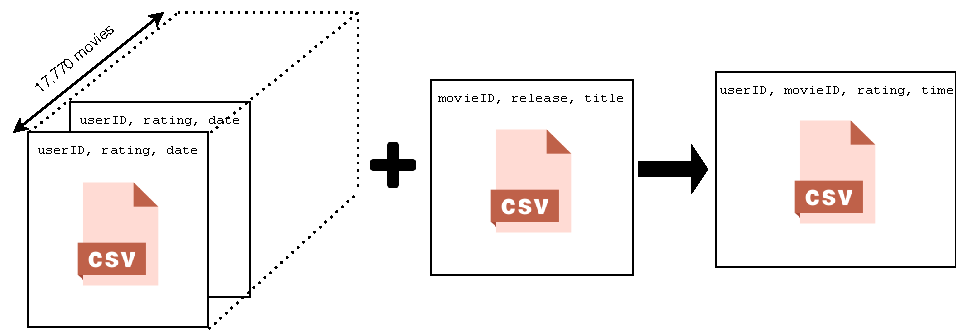
\includegraphics[width=.9\linewidth]{img/processing.pdf}
	\caption{Data reshaping of the Netflix dataset.}
	\label{fig:nf-struct}
\end{figure}

After the reshaping process, useless entries from both database were removed to make the score computation faster later on. Entries can be discarded for different reasons:

\begin{itemize}
	\item Out-of-bounds timestamps: according to its ReadMe, the MovieLens database has records from ratings performed between January 09, 1995 and March 31, 2015. The Netflix database only ranges from October 1998 to December 2005, so that many ratings can be eliminated. The amount of distinct users from MovieLens drops from 138,493 to 52,875.
	
	\item Isolated movie: a movie rating is removed from one database if the movie is not present in the other database as it would not taken into account in the scoring function. A movie was identified by its title and release date to filter only those appearing in both datasets\footnote{Few special cases were also discarded, for example the fact that two movies named \textit{Hamlet} were released in 2000, so that it was not possible to differentiate between them.}. There were around 5800 movies that were rated in both datasets (from the original 17,700 of Netflix).
\end{itemize}

Ultimately, the movie IDs needed to be made consistent between the two datasets to allow for proper implementation of the scoring function. Indeed, movies were not given the same \texttt{movieID} in both datasets.

Those lengthy data manipulations are not de-anonymization \textit{per se} but are an unavoidable step needed to allow the implementation of the algorithm.

% Cédric
\section[]{Results}
\section{Results}\label{sec:results}

\subsection{Matching algorithm}

The matching algorithm was run on subsets of the cleaned MovieLens and Netflix datasets. In total, the subsets included around 3,600 Netflix users and 3,000 MovieLens users (more was not possible due to limited computing power). The algorithm found matches with an eccentricity higher than 1.5 for 819 pairs of users, and an histogram of the results is depicted in \autoref{fig:hist_matches}.

\begin{figure}[h]
	\centering
	\begin{tikzpicture}

\begin{axis}[%
ybar,
height = .3\textheight,
width=\linewidth,
ylabel=Amount of matches,
ymin = 0,
ymax = 80,
xmin = 1.5,
xmax = 8.5,
xlabel = Eccentricity $\phi$,
]
\addplot +[
	hist={
		bins=56,
	}  
] table [col sep=comma,y index = {0}]{data/matches.csv};
\end{axis}
\end{tikzpicture}%
%\end{document}
	\caption{Histogram of the found matches and their corresponding eccentricity.}
	\label{fig:hist_matches}
\end{figure}

Unsurprisingly, most of the identified matches have a low $\phi$ regardless of being above the threshold. More than half the amount of matches have an eccentricity $\phi < 2.5$, casting reasonable doubt about the fact that those are indeed matching users. It is likely that the proposed threshold of 1.5 is too low for the used data. However, 5 matches have an eccentricity of more than 7, for which the belief that de-anonymization was correctly carried out is more plausible.

\subsection{Validation and discussion}

In order to be able to conclude that de-anonymization is successful without the knowledge of the ground truth of matching users, a validation procedure is needed. It is proposed to include a dummy user in both database, with the same ratings and same timestamps for 30 movies. A functioning algorithm should identify a very strong match between the two entries.

This was done for our algorithm and the movies were randomly chosen. The results were averaged over 100 realizations (because the popularity of the involved movies has an impact on the scoring function) and the found match had a mean eccentricity of 60.47. This confirms that entries that match perfectly yield a very high eccentricity. However, such a perfect situation is not expected. Some variability is present in the data, would it be due to user behavior or to noise voluntarily added in the datasets for anonymity purposes. Hence, the robustness to noise is studied later.

An interesting factor influencing the scoring function is the amount of movies that are common for users in both databases. In the validation step, 30 common movies were injected in the data. However, this is a purely arbitrary value. The impact of the number of movies is depicted in \autoref{fig:n_movies}.

\begin{figure}[h]
	\centering
	\begin{tikzpicture}

\begin{axis}[%
height = .3\textheight,
width=\linewidth,
ylabel=Eccentricity $\phi$,
ymin = 0,
ymax = 30,
xmin = 0,
xmax = 30,
xlabel = Amount of common movies,
]
\addplot [blue, only marks] table [col sep=comma,y index = {0}, x expr=\coordindex]{data/n_movies.csv};
\addplot [mark=none, dashed, black] coordinates {(-2,1.5) (32,1.5)};
\end{axis}
\end{tikzpicture}%
%\end{document}
	\caption{Influence of the amount of common movies on the eccentricity of a match. The dashed line highlights the $\phi = 1.5$ threshold.}
	\label{fig:n_movies}
\end{figure}

From this analysis, it can be seen that a single rating that has exactly the same values for $\rho$ and $d$ is enough to exceed the threshold $\phi = 1.5$. However, it is intuitively not enough to conclude that the accounts can be linked together, confirming the hypothesis that the previously found matches with $\phi$ around 2 are not to be trusted.

\subsection{Robustness analysis}

Because noise is present in the data, the same dummy user is used to assess the noise robustness of the scoring function. Instead of including exactly matching records, the ratings and timestamps will be perturbed with uniformly distributed noise. If a movie rating in one database is $\rho$, the corresponding rating in the other database is:

\begin{equation}
	\rho_{\text{noisy}} = \rho + \mathcal{U}\left[-\sigma_{\rho}, \sigma_{\rho}\right]
\end{equation}

Where $\mathcal{U}\left[-\sigma_{\rho}, \sigma_{\rho}\right]$ is a random variable uniformly distributed between $-\sigma_{\rho}$ and $\sigma_{\rho}$. The impact of the rating spread $\sigma_{\rho}$ on the eccentricity of the dummy user is shown in \autoref{fig:noise_rating}, where the eccentricity was again computed as a mean over 100 realizations.

\begin{figure}[h]
	\centering
	\begin{tikzpicture}

\begin{axis}[%
height = .3\textheight,
width=\linewidth,
ylabel=Eccentricity $\phi$,
%ymin = 0,
%ymax = 30,
xmin = 0,
xmax = 5,
xlabel = Rating spread $\sigma_{\rho}$,
]
\addplot [blue, only marks] table [col sep=comma,y index = {1}, x index = {0}]{data/noisy_ratings.csv};
\end{axis}
\end{tikzpicture}%
%\end{document}
	\caption{Influence of noisy movie ratings on the eccentricity of a match.}
	\label{fig:noise_rating}
\end{figure}

Similarly, noise on the rating timestamp is introduced as:

\begin{equation}
d_{\text{noisy}} = d + \mathcal{U}\left[-\sigma_{d}, \sigma_{d}\right]
\end{equation}

The impact of the timestamp spread $\sigma_{d}$ on the eccentricity of the dummy user is shown in \autoref{fig:noise_ts}.

\begin{figure}[h]
	\centering
	\begin{tikzpicture}

\begin{axis}[%
height = .45\textheight,
width=\linewidth,
ylabel=Eccentricity $\phi$,
%ymin = 0,
%ymax = 30,
xmin = 0,
xmax = 90,
xlabel = Timestamp spread $\sigma_{d}$,
]
\addplot [blue, only marks] table [col sep=comma,y index = {1}, x index = {0}]{data/noisy_dates.csv};
\end{axis}
\end{tikzpicture}%
%\end{document}
	\caption{Influence of noisy timestamps on the eccentricity of a match.}
	\label{fig:noise_ts}
\end{figure}

These Figures highlight the fact that the eccentricity is still at a significantly high value in the presence of noise on the input data $\rho$ and $d$. It can be concluded that the metric having the most influence on the eccentricity is the amount of common movies for the two considered users. Regardless of the ratings and timestamps, two profiles are likely to be linked if they share reviews for several unpopular movies and either the rating or the timestamp is corresponding.

\end{document}